\documentclass{beamer}

\usefonttheme{professionalfonts} % using non standard fonts for beamer
\usefonttheme{serif} % default family is serif

\usepackage{enumitem}
\setitemize{label=\usebeamerfont*{itemize item}%
  \usebeamercolor[fg]{itemize item}
  \usebeamertemplate{itemize item}}

\usepackage{hyperref}
%\usepackage{minted}
\usepackage{animate}
\usepackage{graphicx}
\def\Put(#1,#2)#3{\leavevmode\makebox(0,0){\put(#1,#2){#3}}}
\usepackage{colortbl}
\usepackage{tikz}
\usepackage{amssymb}
\usepackage{enumerate}
\usepackage{arydshln}
\usepackage{algorithm}
\usepackage{algpseudocode}

\colorlet{lightred}{red!25}
\colorlet{lightgreen}{green!25}
\beamertemplatenavigationsymbolsempty

\newcommand\blfootnote[1]{%
  \begingroup
  \renewcommand\thefootnote{}\footnote{#1}%
  \addtocounter{footnote}{-1}%
  \endgroup
}

\makeatletter

%% Textclass specific LaTeX commands.
\newcommand\makebeamertitle{\frame{\maketitle}}%
\AtBeginDocument{%
  \let\origtableofcontents=\tableofcontents
  \def\tableofcontents{\@ifnextchar[{\origtableofcontents}{\gobbletableofcontents}}
  \def\gobbletableofcontents#1{\origtableofcontents}
}
%% User specified LaTeX commands.
\usetheme{Malmoe}
\useoutertheme{infolines}
\addtobeamertemplate{headline}{}{\vskip2pt}
\setbeamercovered{transparent}

\makeatother

%%%%%%%%%%%%%%%%%%%%%%%%%%%%%%%%%%%%%%
%% Main document
%%%%%%%%%%%%%%%%%%%%%%%%%%%%%%%%%%%%%%
\begin{document}
\title[PFLOCK report]{PFLOCK Report}
\author[AC]{Andres Calderon}
\institute[Fall'20]{University of California, Riverside}
\makebeamertitle
\newif\iflattersubsect

\AtBeginSection[] {
    \begin{frame}<beamer>
    \frametitle{Outline} 
    \tableofcontents[currentsection]  
    \end{frame}
    \lattersubsectfalse
}

\AtBeginSubsection[] {
    \begin{frame}<beamer>
    \frametitle{Outline} 
    \tableofcontents[currentsubsection]  
    \end{frame}
}

\begin{frame}{A mistake in my previous approach...}
    \centering
    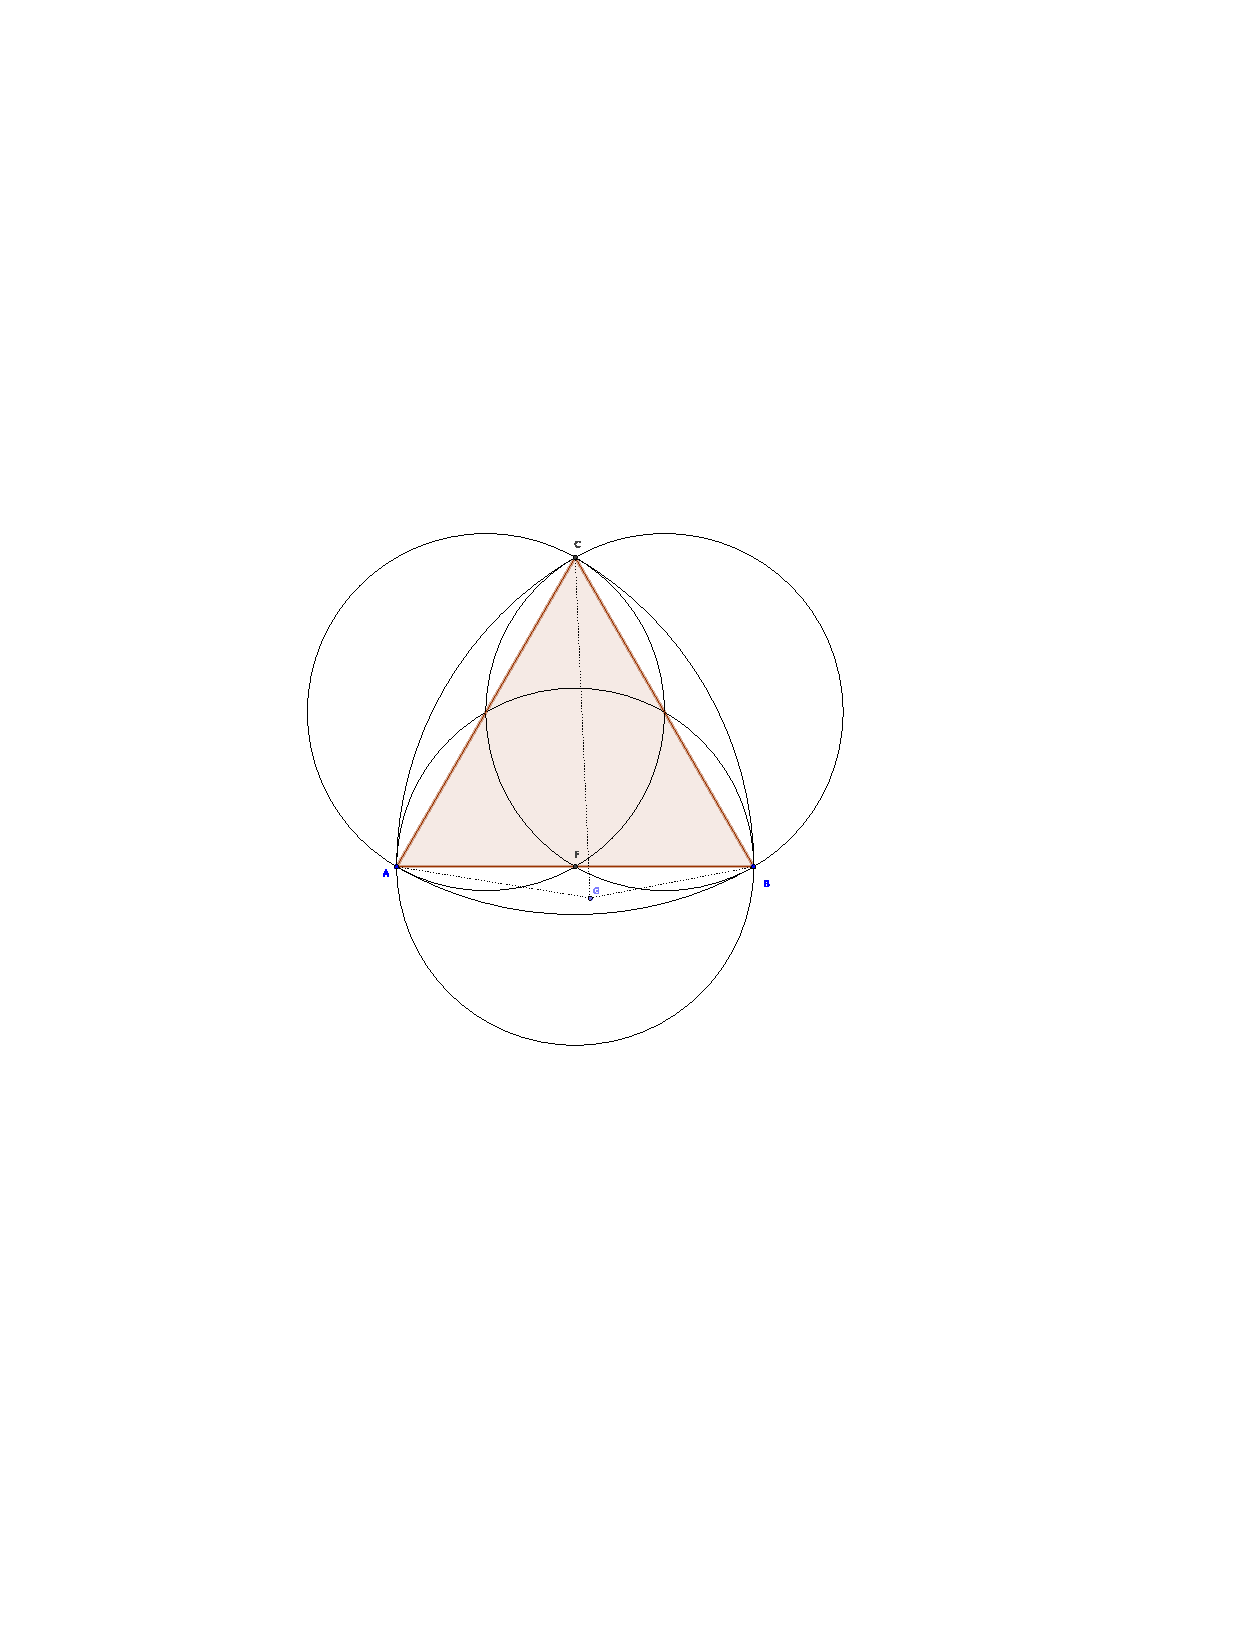
\includegraphics[trim=2cm 8cm 2cm 8cm,clip,width=1\textwidth]{figures/Mistake}
\end{frame}

\begin{frame}{Can still MBC help?}{Extremal points}
    \begin{itemize}
        \item The 3 points which describe the MBC in an input set of points...
    \end{itemize}
    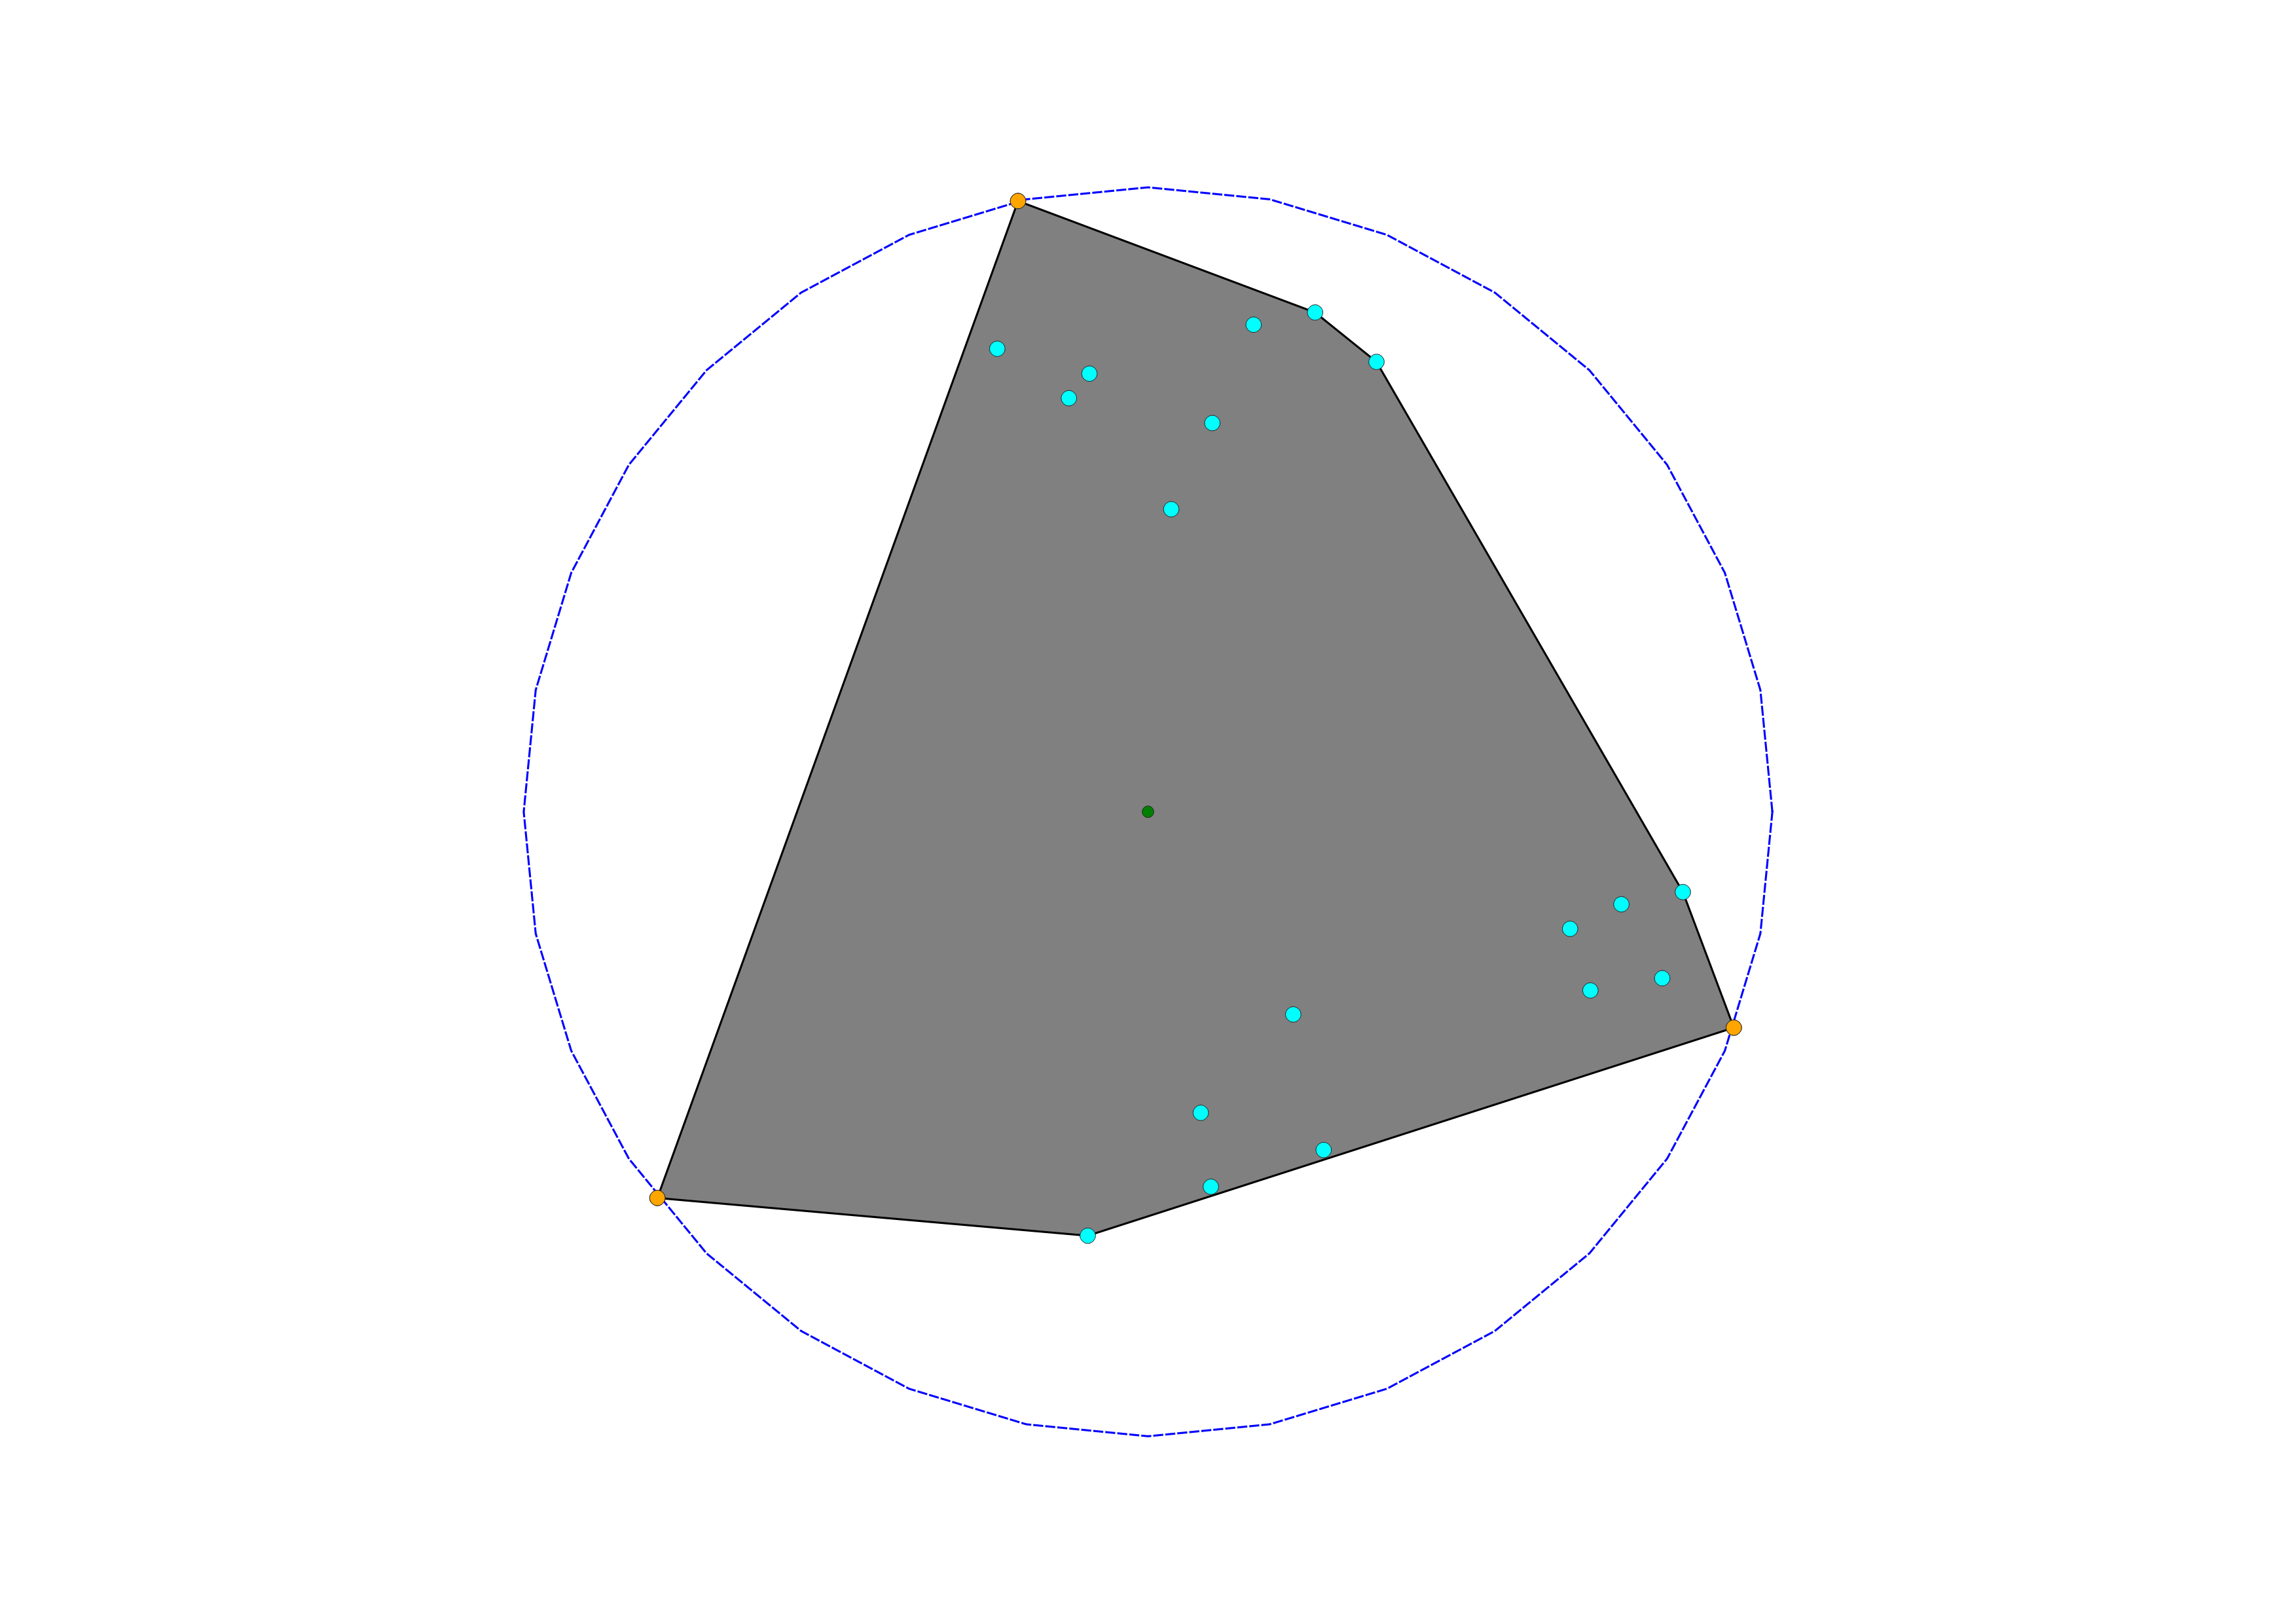
\includegraphics[width=0.9\textwidth]{figures/Extremal_4}
\end{frame}

\begin{frame}{Can still MBC help?}{Extremal points}
    \centering
    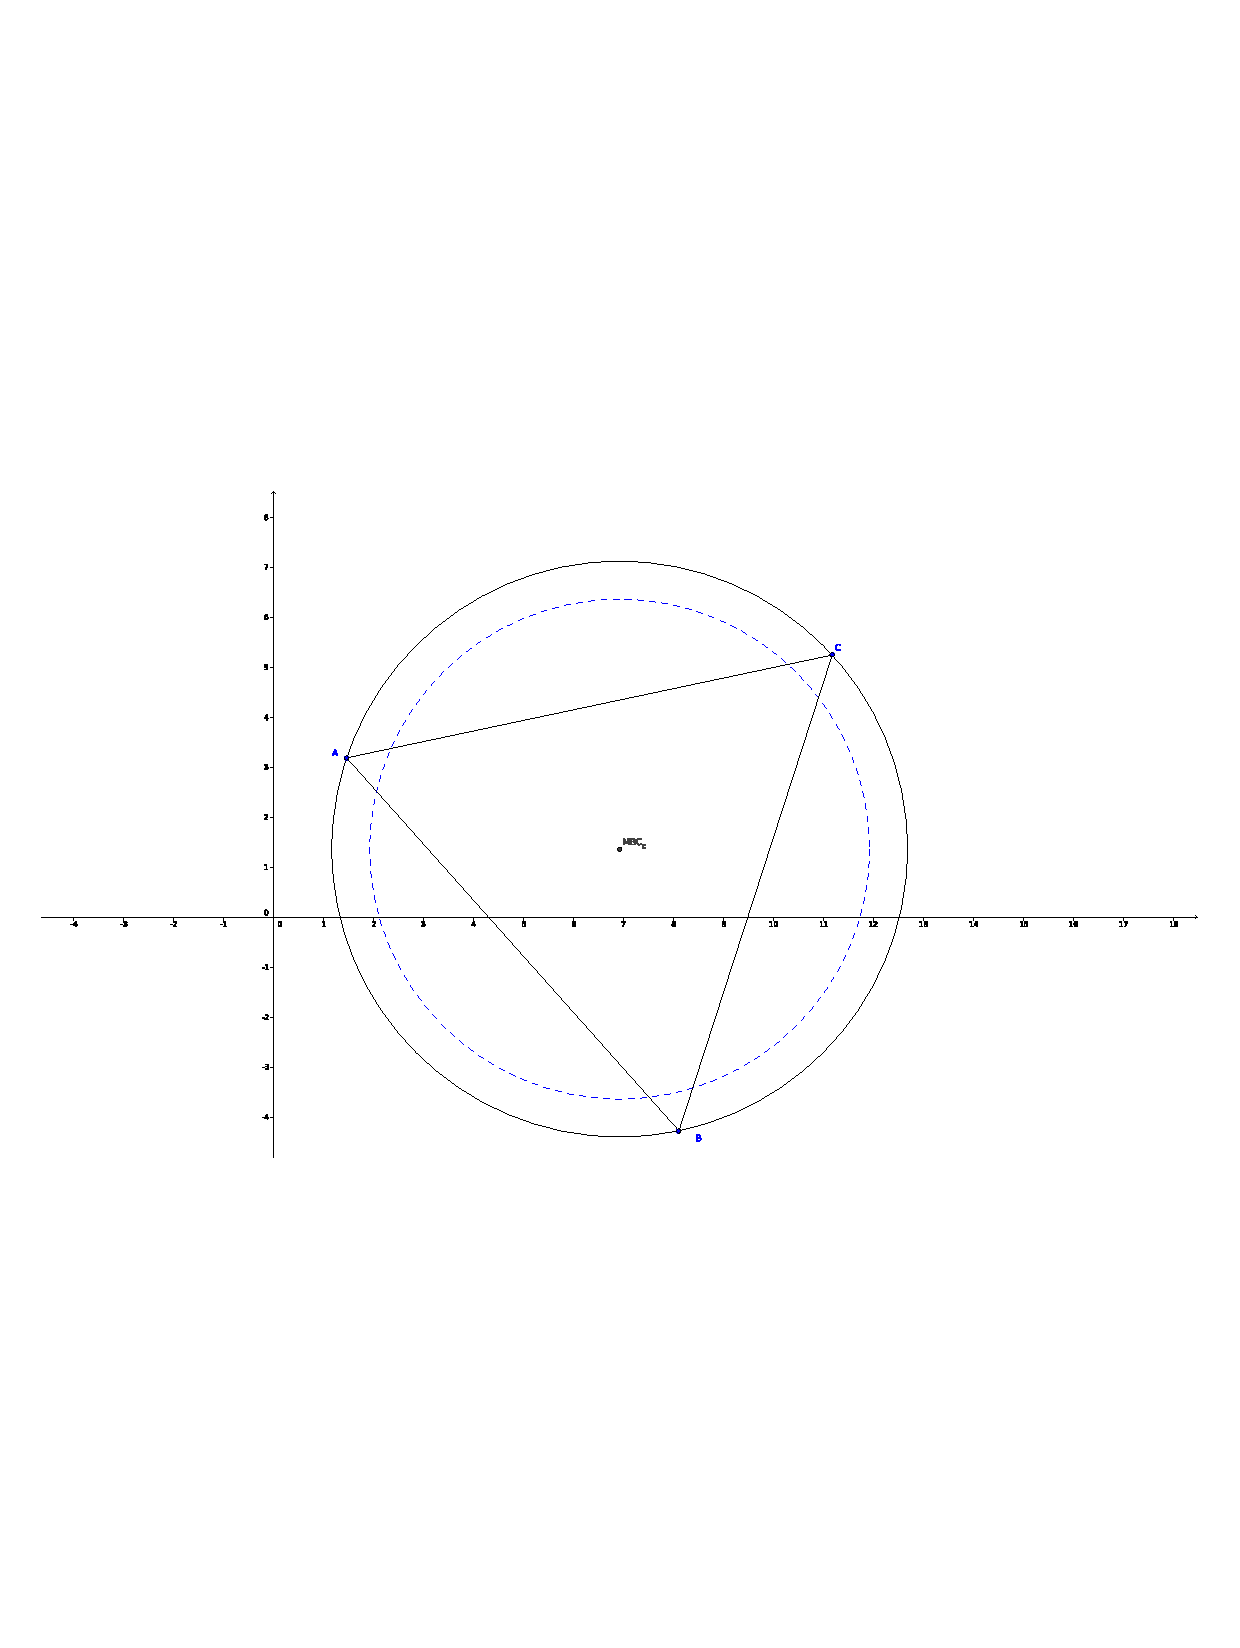
\includegraphics[trim=2cm 8cm 2cm 8cm,clip,width=0.8\textwidth]{figures/MBCs}
\end{frame}

\begin{frame}{Proposed Algorithm}
    \begin{itemize}
        \item Input: Maximal cliques which MBC is greater than $\epsilon$
    \end{itemize}
    For each clique:
    \begin{enumerate}[label*=\arabic*.]
        \item $P \leftarrow $ Set of points in clique
        \item $S \leftarrow \emptyset$
        \item Find $MBC$ in $P$
        \item While $MBC.radius <= \frac{\epsilon}{2}$:
        \begin{enumerate}[label*=\arabic*.]
            \item $E \leftarrow ExtremalPoints(MBC)$ 
            \item $S \leftarrow S \cup E$
            \item $P \leftarrow P - E$
            \item Find $MBC$ in $P$
        \end{enumerate}
        \item $S \leftarrow S \cup ConvexHull(P)$
        \item return $S$
    \end{enumerate}
\end{frame}

\begin{frame}{What's next}
    \begin{itemize}
        \item I have implemented the algorithm and the output compared with the previous implementation are the same.
        \item Still working on the formal proof.
        \item Run performance tests with more datasets.
    \end{itemize}

\end{frame}

\end{document}

